
The system is divided into three parts, frontend, Tester and backend with the database. Tester whose main task is to implement a system that is able to test code that students write and send back the response of the tests. The frontend should visualize the user interface and the gamification parts. The backend is the in the middle and it will forward the code from frontend and load a test from the database, then send the submitted code along with the tests to Tester and then handle the response back to the frontend. The decision of what programming language to use was based on the following criteria, it should be fullstack meaning the same language should be used in all the parts for easier collaboration between the software engineers, it should be suitable for web and it should be fairly modern programming language. The two alternatives found was Python with frameworks or JavaScript with frameworks. The chosen programming language was JavaScript using Node.Js for backend and Tester, MongoDB as a NoSQL database and Angular4 for frontend.
\begin{figure}[hb]
    \centering
    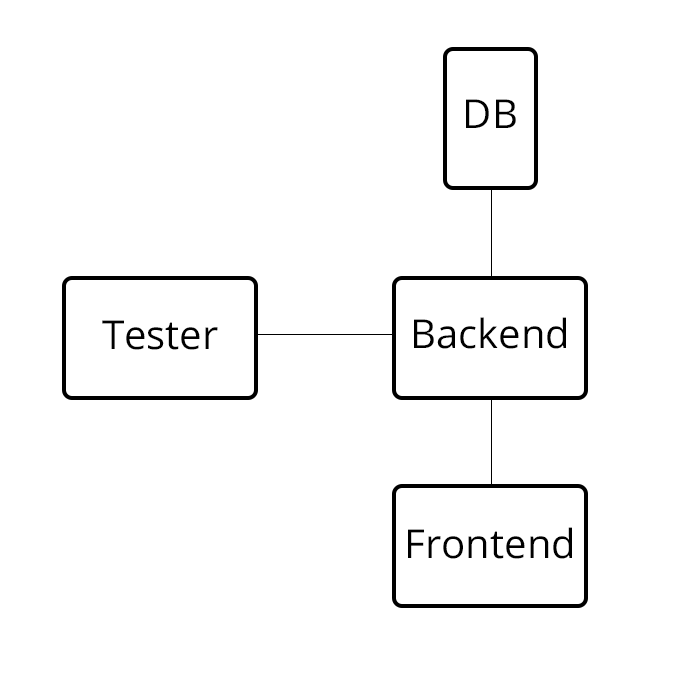
\includegraphics[scale=0.4]{img/SystemA2.png}
    \caption{A simple sketch over the system parts and how they are connected.}
\end{figure}
